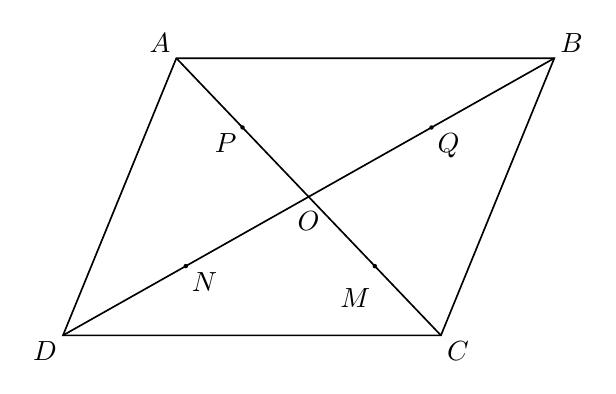
\begin{tikzpicture}[x=1cm,y=1cm,font=\normalsize,
 geometry edge/.style={solid,line width=.6pt},
 geometry mark/.style={solid,line width=.6pt},
 geometry label/.style={font=\normalsize,inner sep=2pt}]
\coordinate (A) at (1.440000000,3.520000000);
\coordinate (B) at (6.240000000,3.520000000);
\coordinate (C) at (4.800000000,0.000000000);
\coordinate (D) at (0.000000000,0.000000000);
\coordinate (O) at (3.120000000,1.760000000);
\coordinate (P) at (2.280000000,2.640000000);
\coordinate (Q) at (4.680000000,2.640000000);
\coordinate (M) at (3.960000000,0.880000000);
\coordinate (N) at (1.560000000,0.880000000);
\draw[geometry edge] (A)--(B)--(C)--(D)--cycle;
\draw[geometry edge] (A)--(P)--(O)--(M)--(C);
\draw[geometry edge] (B)--(Q)--(O)--(N)--(D);
\node[geometry label,above left] at (A) {$A$};
\node[geometry label,above right] at (B) {$B$};
\node[geometry label,below right] at (C) {$C$};
\node[geometry label,below left] at (D) {$D$};
\node[geometry label,below,yshift=-3pt] at (O) {$O$};
\node[geometry label,below left] at (P) {$P$};
\node[geometry label,below right] at (Q) {$Q$};
\node[geometry label,below,xshift=-7pt,yshift=-6pt] at (M) {$M$};
\node[geometry label,below right] at (N) {$N$};
\fill (P) circle[radius=.8pt];
\fill (Q) circle[radius=.8pt];
\fill (M) circle[radius=.8pt];
\fill (N) circle[radius=.8pt];
\end{tikzpicture}